\documentclass[11pt]{article}
\usepackage[left=2cm,right=2cm]{geometry}
\usepackage[font=scriptsize]{caption}
\usepackage{titlesec}
\usepackage{float}
\usepackage{graphicx}
\usepackage{lineno}
\usepackage{cite}
\titleformat*{\section}{\large\bfseries}

\title{Project Proposal: Understanding the Spread of Zoonotic Diseases Caused by Alien Invasive Species}

\author{Cherie Yu} 

\date{3 December 2021\linebreak Supervisor Names: David Redding(External), Will Pearse(Internal)\linebreak Email: david.redding@ioz.ac.uk, will.pearse@imperial.ac.uk \linebreak Affiliations: Zoological Society of London, University of Exeter}

\linespread{1.25}
\begin{document}
\maketitle

\pagebreak
\noindent\textbf{Keywords:} Zoonotic Diseases, Invasive Species, Global Changes, Trade Networks, Climate Change, Host Pathogen Dynamics 

\linenumbers
\noindent\textbf{Introduction} 

The recent Covid-19 pandemic has brought back awareness to the threats of zoonotic diseases on human and biodiversity 
health \cite{stephens_characteristics_2021,tedeschi_introduction_nodate}. 
Zoonotic disease results from the cross-species transmission of pathogens between wildlife, domesticated animals 
and humans and are estimated to be 70\% of the majority of emerging human disease \cite{stephens_characteristics_2021,tedeschi_introduction_nodate}. 
Global changes are expected to increase the mixing of humans and wildlife from previously unconnected communities, increasing the emergence of novel pathogens 
\cite{glidden_human-mediated_2021,chapman_global_2017,michael_r_lelimini_invasive_2021,robinson_double_2020,pysek_scientists_2020,ogden_emerging_nodate}.
Our definition of species invasions is the introduction of species into an environment outside of their normal ranges, through 
human-mediated movement \cite{chinchio_invasive_2020}. This is a growing concern as invasive alien species has been listed as a 
major indicator of global biodiversity decline \cite{pysek_scientists_2020,michael_r_lelimini_invasive_2021}. Invasive species 
can act as vectors or reservoir hosts for pathogens. They can also bring in new pathogens that alter disease dynamics \cite{glidden_human-mediated_2021}. Greater understanding is 
needed on how invasive species are spread, transported and introduced through human movements, helping to form global management 
solutions \cite{schindler_alien_2015}. In addition, there is a lack of comprehensive data on pathogens hosted and spread by 
invasive alien species \cite{chinchio_invasive_2020}. It is not known how future 
introductions of alien species might lead to changes in zoonotic risk patterns. For instance, anthropogenic transport networks 
are predicted to be influential on the alteration of the geographic spread of species \cite{chapman_global_2017}. 
In this study, we will be using large databases to examine host-pathogen interactions and human-animal introductions, exploring these questions: 
1) What are the characteristics of species that are both successfully invasive and 
are host species? 2) By tracking the movement of invasives by human translocation, which areas 
are more at risk to zoonotic diseases? 3) Can we identify how disease transmission have been heighten with the introduction of invasive species into new areas? 

\noindent\textbf{Proposed Methods}

\noindent1) First, I will use database methods to create a joint database describing which species groups
are invasive, disease-carrying and both invasive and disease carrying. Using simulations, I will 
ask whether the relative size of these groups can be explained by random processes and then use phylogenies 
to see how evolutionarily conserved these traits are. Finally, I will use phylogenetic least squares 
regressions to identify what makes those species successful at being both invasive and disease hosts, for 
example, body size, life history, food generalist or habitat preferences.

\noindent2) Here, I will first create a map of propagule pressure, showing which areas of the world have the high density of potential 
invasive host species. I will then create a map of all invasive species that have invaded new areas of the world but are not
within the current endemic range of the diseases they carry. Then I will use free available networks of the human 
transport to identify, via simulation, which areas are at highest risk of future zoonotic disease spread. 

\noindent3) Lastly, I will look at the role of species introduced to areas outside their range and using estimates of population 
densities and habitat preferences, for these introduced species and employ disease transmission models to identify how 
disease transmission have been heighten with the introduction of new invasives around people? 

\noindent\textbf{Anticipated Outputs and Outcomes}

Our results can be used to predict and formulate future management strategies in regulating zoonotic disease outbreak. Current legislations by 
the World Trade Organization are in placed to secure trades in wildlife that minimizes introduction of parasites 
however, international wildlife trade regulations pay less attention to the risk of establishment of invasive 
species in the wild \cite{hulme_invasive_2014}. I anticipate that my results will show a significant overlap between invasive 
species that are also zoonotic hosts. In addition, alien species thrive in anthropogenic environments that increase 
risk of transmission to humans \cite{hulme_invasive_2014}. Globalization has intensified the amount of introduced taxa from
different origins, climates and habitats, increasing the likelihood of virus host jumps, hybridization and evolutionary 
change \cite{hulme_invasive_2014}. I also anticipate that alien species with faster, shorter life history traits have a higher
change to act as host reservoirs \cite{keesing_impacts_2021}. 

\noindent\textbf{Gannt Chart}

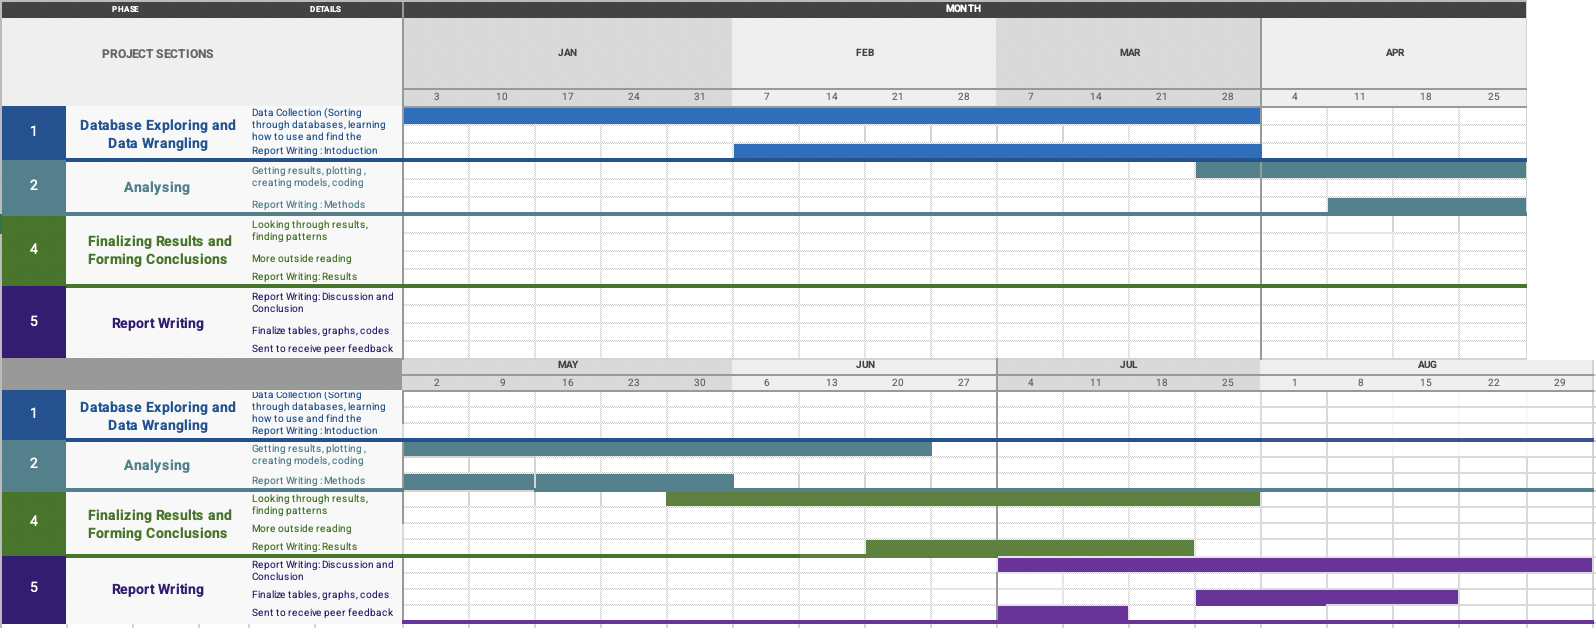
\includegraphics[scale=0.5]{test} 

\noindent\textbf{Budget}

£250 is suggested for the project budget to gain access to books, online materials and learning packages for computational 
techniques, get a hard drive, computing time on the cluster. 

\pagebreak
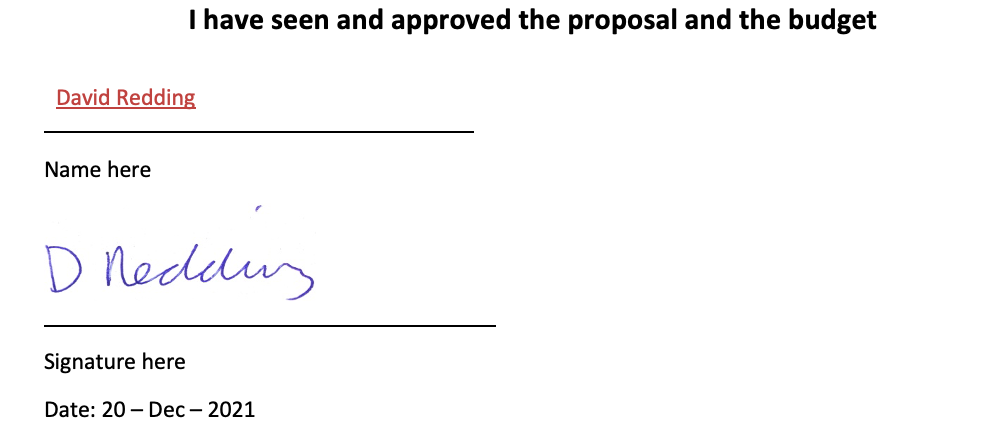
\includegraphics[scale=0.5]{sign}

\bibliographystyle{apalike}
\nolinenumbers
\bibliography{Project_Proposal}
\end{document}